% Options for packages loaded elsewhere
% Options for packages loaded elsewhere
\PassOptionsToPackage{unicode}{hyperref}
\PassOptionsToPackage{hyphens}{url}
\PassOptionsToPackage{dvipsnames,svgnames,x11names}{xcolor}
%
\documentclass[
  oneside,
  open=any,
  fontsize=11pt]{article}
\usepackage{xcolor}
\usepackage{amsmath,amssymb}
\setcounter{secnumdepth}{-\maxdimen} % remove section numbering
\usepackage{iftex}
\ifPDFTeX
  \usepackage[T1]{fontenc}
  \usepackage[utf8]{inputenc}
  \usepackage{textcomp} % provide euro and other symbols
\else % if luatex or xetex
  \usepackage{unicode-math} % this also loads fontspec
  \defaultfontfeatures{Scale=MatchLowercase}
  \defaultfontfeatures[\rmfamily]{Ligatures=TeX,Scale=1}
\fi
\usepackage{lmodern}
\ifPDFTeX\else
  % xetex/luatex font selection
\fi
% Use upquote if available, for straight quotes in verbatim environments
\IfFileExists{upquote.sty}{\usepackage{upquote}}{}
\IfFileExists{microtype.sty}{% use microtype if available
  \usepackage[]{microtype}
  \UseMicrotypeSet[protrusion]{basicmath} % disable protrusion for tt fonts
}{}
\makeatletter
\@ifundefined{KOMAClassName}{% if non-KOMA class
  \IfFileExists{parskip.sty}{%
    \usepackage{parskip}
  }{% else
    \setlength{\parindent}{0pt}
    \setlength{\parskip}{6pt plus 2pt minus 1pt}}
}{% if KOMA class
  \KOMAoptions{parskip=half}}
\makeatother
% Make \paragraph and \subparagraph free-standing
\makeatletter
\ifx\paragraph\undefined\else
  \let\oldparagraph\paragraph
  \renewcommand{\paragraph}{
    \@ifstar
      \xxxParagraphStar
      \xxxParagraphNoStar
  }
  \newcommand{\xxxParagraphStar}[1]{\oldparagraph*{#1}\mbox{}}
  \newcommand{\xxxParagraphNoStar}[1]{\oldparagraph{#1}\mbox{}}
\fi
\ifx\subparagraph\undefined\else
  \let\oldsubparagraph\subparagraph
  \renewcommand{\subparagraph}{
    \@ifstar
      \xxxSubParagraphStar
      \xxxSubParagraphNoStar
  }
  \newcommand{\xxxSubParagraphStar}[1]{\oldsubparagraph*{#1}\mbox{}}
  \newcommand{\xxxSubParagraphNoStar}[1]{\oldsubparagraph{#1}\mbox{}}
\fi
\makeatother


\usepackage{longtable,booktabs,array}
\usepackage{calc} % for calculating minipage widths
% Correct order of tables after \paragraph or \subparagraph
\usepackage{etoolbox}
\makeatletter
\patchcmd\longtable{\par}{\if@noskipsec\mbox{}\fi\par}{}{}
\makeatother
% Allow footnotes in longtable head/foot
\IfFileExists{footnotehyper.sty}{\usepackage{footnotehyper}}{\usepackage{footnote}}
\makesavenoteenv{longtable}
\usepackage{graphicx}
\makeatletter
\newsavebox\pandoc@box
\newcommand*\pandocbounded[1]{% scales image to fit in text height/width
  \sbox\pandoc@box{#1}%
  \Gscale@div\@tempa{\textheight}{\dimexpr\ht\pandoc@box+\dp\pandoc@box\relax}%
  \Gscale@div\@tempb{\linewidth}{\wd\pandoc@box}%
  \ifdim\@tempb\p@<\@tempa\p@\let\@tempa\@tempb\fi% select the smaller of both
  \ifdim\@tempa\p@<\p@\scalebox{\@tempa}{\usebox\pandoc@box}%
  \else\usebox{\pandoc@box}%
  \fi%
}
% Set default figure placement to htbp
\def\fps@figure{htbp}
\makeatother





\setlength{\emergencystretch}{3em} % prevent overfull lines

\providecommand{\tightlist}{%
  \setlength{\itemsep}{0pt}\setlength{\parskip}{0pt}}



 


\usepackage{booktabs}
\usepackage{longtable}
\usepackage{array}
\usepackage{multirow}
\usepackage{wrapfig}
\usepackage{float}
\usepackage{colortbl}
\usepackage{pdflscape}
\usepackage{tabu}
\usepackage{threeparttable}
\usepackage{threeparttablex}
\usepackage[normalem]{ulem}
\usepackage{makecell}
\usepackage{xcolor}
\usepackage{geometry}
\usepackage{pdflscape}
\usepackage{afterpage}
\usepackage{graphicx}
\usepackage{float}
\usepackage{array}
\usepackage{booktabs}
\usepackage{longtable}
\usepackage{multirow}
\usepackage{wrapfig}
\usepackage{colortbl}
\usepackage{pdflscape}
\usepackage{tabu}
\usepackage{threeparttable}
\usepackage{threeparttablex}
\usepackage[normalem]{ulem}
\usepackage{makecell}
\usepackage{xcolor}
\makeatletter
\@ifpackageloaded{caption}{}{\usepackage{caption}}
\AtBeginDocument{%
\ifdefined\contentsname
  \renewcommand*\contentsname{Table of contents}
\else
  \newcommand\contentsname{Table of contents}
\fi
\ifdefined\listfigurename
  \renewcommand*\listfigurename{List of Figures}
\else
  \newcommand\listfigurename{List of Figures}
\fi
\ifdefined\listtablename
  \renewcommand*\listtablename{List of Tables}
\else
  \newcommand\listtablename{List of Tables}
\fi
\ifdefined\figurename
  \renewcommand*\figurename{Figure}
\else
  \newcommand\figurename{Figure}
\fi
\ifdefined\tablename
  \renewcommand*\tablename{Table}
\else
  \newcommand\tablename{Table}
\fi
}
\@ifpackageloaded{float}{}{\usepackage{float}}
\floatstyle{ruled}
\@ifundefined{c@chapter}{\newfloat{codelisting}{h}{lop}}{\newfloat{codelisting}{h}{lop}[chapter]}
\floatname{codelisting}{Listing}
\newcommand*\listoflistings{\listof{codelisting}{List of Listings}}
\makeatother
\makeatletter
\makeatother
\makeatletter
\@ifpackageloaded{caption}{}{\usepackage{caption}}
\@ifpackageloaded{subcaption}{}{\usepackage{subcaption}}
\makeatother
\usepackage{bookmark}
\IfFileExists{xurl.sty}{\usepackage{xurl}}{} % add URL line breaks if available
\urlstyle{same}
\hypersetup{
  pdftitle={Strategic Resilience and Financial Performance Profile for Nexperia Germany},
  pdfauthor={Ronald de Boer},
  colorlinks=true,
  linkcolor={blue},
  filecolor={Maroon},
  citecolor={Blue},
  urlcolor={Blue},
  pdfcreator={LaTeX via pandoc}}


\title{Strategic Resilience and Financial Performance Profile for
Nexperia Germany}
\usepackage{etoolbox}
\makeatletter
\providecommand{\subtitle}[1]{% add subtitle to \maketitle
  \apptocmd{\@title}{\par {\large #1 \par}}{}{}
}
\makeatother
\subtitle{An In-depth Analysis by the Supply Chain Finance Lectoraat,
Hogeschool Windesheim}
\author{Ronald de Boer}
\date{}
\begin{document}
\maketitle


\section{PART 5 - STRATEGIC RESILIENCE
DASHBOARD}\label{part-5---strategic-resilience-dashboard}

\newgeometry{left=1cm,right=1cm,top=1.5cm,bottom=1cm}
\thispagestyle{empty}

\begin{center}
\Large\textbf{Strategic Supply Chain Resilience Assessment}\\
\large\textbf{ Nexperia Germany }\\
\small Generated:  September 14, 2025  | SCRES: \textbf{ 2.70 /5.00}\\
\footnotesize Partnership: NextGenResilience • RUG • Windesheim • Involvation\\
\end{center}

\vspace{0.3cm}

\pandocbounded{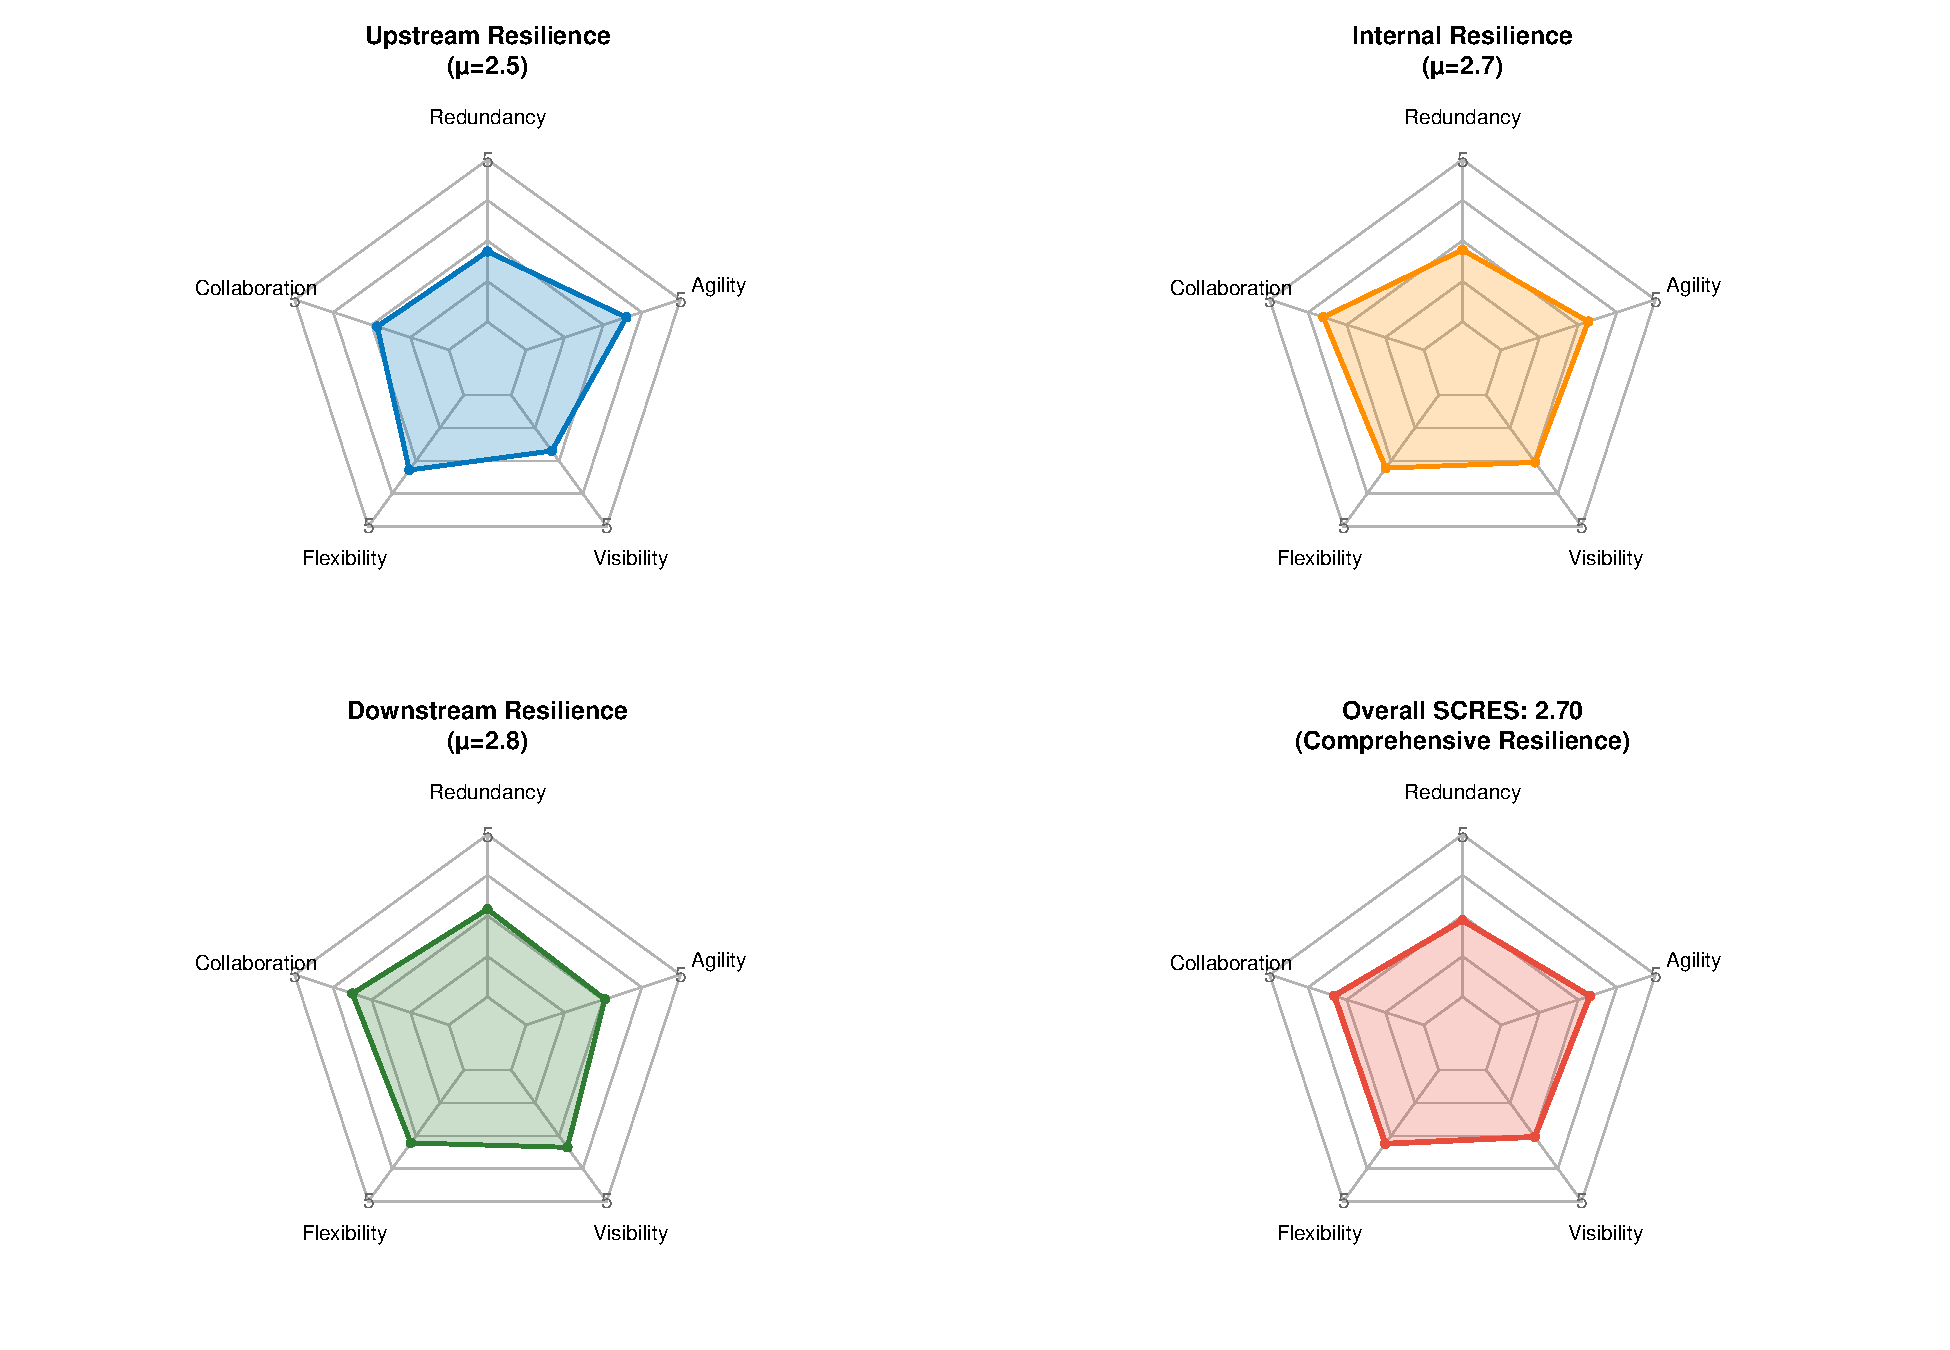
\includegraphics[keepaspectratio]{example_3_files/figure-pdf/main-dashboard-content-1.pdf}}

\vspace{0.4cm}

\begin{minipage}[t]{0.48\textwidth}
\textbf{\large Executive Summary}\\
\textbf{Overall Performance:}  Below Average  ( 2.70 /5.00)\\
\textbf{Strongest Pillar:} Downstream  ( 2.82 )\\
\textbf{Development Area:}  Upstream  ( 2.54 )\\
\textbf{Performance Spread:}  0.28  points\\
\footnotesize\textit{Note: Using deterministic synthetic baseline for demonstration}\\
\end{minipage}\hfill
\begin{minipage}[t]{0.48\textwidth}
\textbf{\large Dutch Language Analysis}\\
\textbf{Upstream:}  Hoogste scores bij Agility, Flexibility; laagste scores bij Redundancy, Visibility \\
\textbf{Internal:}  Hoogste scores bij Collaboration, Agility; laagste scores bij Visibility, Redundancy \\
\textbf{Downstream:}  Hoogste scores bij Collaboration, Visibility; laagste scores bij Redundancy, Agility \\
\end{minipage}

\vspace{0.4cm}

\begin{minipage}[t]{0.32\textwidth}
\textbf{\large Upstream Resilience}\\
\textbf{Focus:} Supplier ecosystem management\\
\textbf{Key Capabilities:} Supplier diversification, contract flexibility, supply risk monitoring, vendor qualification processes. Critical for maintaining input continuity during supplier disruptions.\\
\end{minipage}\hfill
\begin{minipage}[t]{0.32\textwidth}
\textbf{\large Internal Resilience}\\
\textbf{Focus:} Core operational adaptability\\
\textbf{Key Capabilities:} Process flexibility, workforce cross-training, buffer capacity, operational visibility, rapid decision-making. Determines speed of operational adaptation to changing conditions.\\
\end{minipage}\hfill
\begin{minipage}[t]{0.32\textwidth}
\textbf{\large Downstream Resilience}\\
\textbf{Focus:} Customer service continuity\\
\textbf{Key Capabilities:} Distribution flexibility, delivery options, customer communication, demand sensing, service recovery. Protects revenue and customer relationships during disruptions.\\
\end{minipage}

\vspace{0.4cm}

\begin{minipage}[t]{0.58\textwidth}
\textbf{Strategic Recommendations}\\
\footnotesize\textbf{Priority Enhancement Areas:}\\
\textbullet\ \textbf{ Upstream Visibility  ( 2.1 ):} Monitoring systems, analytics, end-to-end transparency\\
\textbullet\ \textbf{ Upstream Redundancy  ( 2.2 ):} Backup suppliers, buffer inventory, alternative routes\\
\textbullet\ \textbf{ Internal Redundancy  ( 2.2 ):} Backup suppliers, buffer inventory, alternative routes\\
\end{minipage}\hfill
\begin{minipage}[t]{0.38\textwidth}
\textbf{Financial Impact}\\
\footnotesize\textbf{Risk Mitigation Value:}\\
\textbullet\ Reduced disruption costs\\
\textbullet\ Lower expediting fees\\
\textbullet\ Improved delivery performance\\
\textbullet\ Enhanced customer retention\\
\textbullet\ Optimized working capital\\
\textbullet\ Competitive reliability advantage\\
\end{minipage}

\vfill
\begin{center}
\footnotesize\textit{Assessment conducted using the Supply Chain Resilience Framework - Supply Chain Finance Lectoraat, Hogeschool Windesheim}
\end{center}




\end{document}
